\documentclass[tikz]{standalone}

\usetikzlibrary{positioning}

\tikzset{node/.style={circle, draw, thick}}
\def\layersep{2}
\def\nodesep{1.5}

\begin{document}
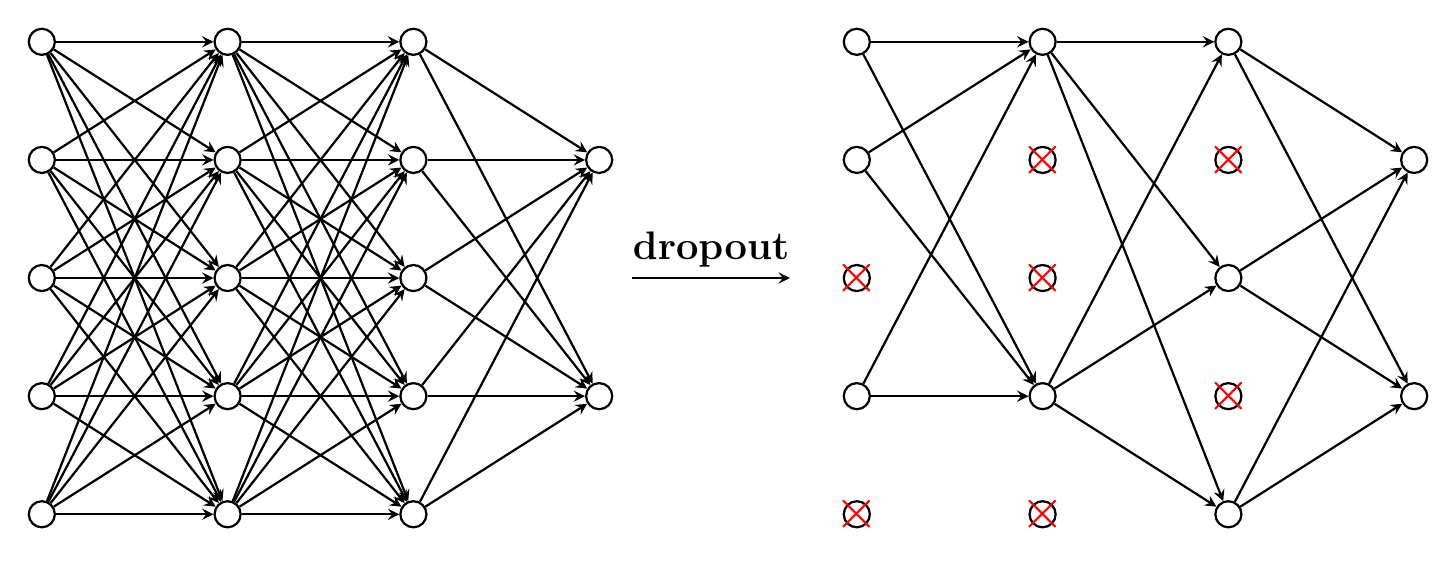
\begin{tikzpicture}

  \foreach \y in {1,...,5}{
      \node[node] (i\y) at (0,\nodesep*\y) {};
      \node[node, right=\layersep of i\y] (h1\y) {};
      \node[node, right=\layersep of h1\y] (h2\y) {};
    }

  \node[node, right=\layersep of h22] (o1) {};
  \node[node, right=\layersep of h24] (o2) {};

  \foreach \source in {1,...,5}
  \foreach \dest in {1,...,5}{
      \path[-stealth, thick] (i\source) edge (h1\dest);
      \path[-stealth, thick] (h1\source) edge (h2\dest);
    }
  \foreach \source in {1,...,5}
  \foreach \dest in {1,2}
  \draw[-stealth, thick] (h2\source) -- (o\dest);

  \draw[-stealth, thick] (7.5,3*\nodesep) -- node[above,font=\Large\bfseries] {dropout} (9.5, 3*\nodesep);

  %%% Boundary %%%

  \foreach \y in {1,...,5}
  \node[node, right=15em of h2\y] (di\y) {};

  \node[red,font=\huge] at (di1) {$\times$};
  \node[red,font=\huge] at (di3) {$\times$};

  \foreach \y in {1,...,5}
  \node[node, right=\layersep of di\y] (dh1\y) {};

  \node[red,font=\huge] at (dh11) {$\times$};
  \node[red,font=\huge] at (dh13) {$\times$};
  \node[red,font=\huge] at (dh14) {$\times$};

  \foreach \y in {1,...,5}
  \node[node, right=\layersep of dh1\y] (dh2\y) {};

  \node[red,font=\huge] at (dh22) {$\times$};
  \node[red,font=\huge] at (dh24) {$\times$};

  \node[node, right=\layersep of dh22] (do1) {};
  \node[node, right=\layersep of dh24] (do2) {};

  \foreach \source in {2,4,5}
  \foreach \dest in {2,5}
  \draw[-stealth, thick] (di\source) -- (dh1\dest);

  \foreach \source in {2,5}
  \foreach \dest in {1,3,5}
  \draw[-stealth, thick] (dh1\source) -- (dh2\dest);

  \foreach \source in {1,3,5}
  \foreach \dest in {1,2}
  \draw[-stealth, thick] (dh2\source) -- (do\dest);
\end{tikzpicture}
\end{document}